\documentclass[../psets.tex]{subfiles}

\pagestyle{main}
\renewcommand{\leftmark}{Problem Set 1}

\begin{document}




\begin{enumerate}[label={\Roman*)}]
    \item \marginnote{1/21:}Do the following (VSEPR) problems from your text (Miessler et al. (2014)): Chapter 3: \#8, 9f-i, 20, 29.
    \begin{enumerate}[label={\textbf{3.\arabic*}}]
        \setcounter{enumii}{7}
        \item Give Lewis dot structures and sketch the shapes of the following:
        \begin{enumerate}[label={\textbf{\alph*.}}]
            \item \ce{SeCl4}
            \begin{center}
                \vspace{1em}
                \chemfig{\charge{45=\:}{Se}(-\charge{0=\:,90=\:,-90=\:}{Cl})(-[2]\charge{0=\:,90=\:,180=\:}{Cl})(-[4]\charge{-90=\:,90=\:,180=\:}{Cl})-[6]\charge{0=\:,-90=\:,180=\:}{Cl}}
                \hspace{3cm}
                \chemfig{Se(-\Charge{0=\:}{})(-[2]Cl)(-[6]Cl)(>:[:160]Cl)(<[:-150]Cl)}
                \vspace{1em}
            \end{center}
            \item \ce{I3-}
            \begin{center}
                \vspace{1em}
                \chemleft{[}
                    \chemfig{\charge{90=\:,180=\:,270=\:}{I}-\charge{90=\:,270=\:}{I}-\charge{90=\:,0=\:,-90=\:}{I}}
                \chemright{]^{-}}
                \hspace{3cm}
                \chemfig{I-[1]\charge{45=\:,135=\:}{I}-[7]I}
                \vspace{1em}
            \end{center}
            \item \ce{PSCl3}
            \begin{center}
                \vspace{1em}
                \chemfig{P(=\charge{45=\:,-45=\:}{S})(-[2]\charge{0=\:,90=\:,180=\:}{Cl})(-[4]\charge{-90=\:,90=\:,180=\:}{Cl})-[6]\charge{0=\:,-90=\:,180=\:}{Cl}}
                \hspace{3cm}
                \chemfig{P(-[:-30]Cl)(<[:-110]Cl)(>:[:-150]Cl)=[2]S}
                \vspace{1em}
            \end{center}
            \item \ce{IF4-}
            \begin{center}
                \vspace{1em}
                \chemleft{[}
                    \chemfig{\charge{45=\:,-135=\:}{I}(-\charge{-90=\:,0=\:,90=\:}{F})(-[2]\charge{0=\:,90=\:,180=\:}{F})(-[4]\charge{90=\:,180=\:,270=\:}{F})-[6]\charge{0=\:,180=\:,270=\:}{F}}
                \chemright{]^{-}}
                \hspace{3cm}
                \chemfig{I(>:[:30]F)(-[2]\charge{90=\:}{})(>:[:150]F)(<[:-150]F)(-[6]\charge{-90=\:}{})<[:-30]F}
                \vspace{1em}
            \end{center}
            \item \ce{PH2-}
            \begin{center}
                \vspace{1em}
                \chemleft{[}
                    \chemfig{H-\charge{90=\:,270=\:}{P}-H}
                \chemright{]^{-}}
                \hspace{3cm}
                \chemfig{H-[1]\charge{45=\:,135=\:}{P}-[7]H}
                \vspace{1em}
            \end{center}
            \item \ce{TeF4^2-}
            \begin{center}
                \vspace{1em}
                \chemleft{[}
                    \chemfig{\charge{45=\:,-135=\:}{Te}(-\charge{-90=\:,0=\:,90=\:}{F})(-[2]\charge{0=\:,90=\:,180=\:}{F})(-[4]\charge{90=\:,180=\:,270=\:}{F})-[6]\charge{0=\:,180=\:,270=\:}{F}}
                \chemright{]^{2-}}
                \hspace{3cm}
                \chemfig{Te(>:[:30]F)(-[2]\charge{90=\:}{})(>:[:150]F)(<[:-150]F)(-[6]\charge{-90=\:}{})<[:-30]F}
                \vspace{1em}
            \end{center}
            \item \ce{N3-}
            \begin{center}
                \vspace{1em}
                \chemleft{[}
                    \chemfig{\charge{135=\:,-135=\:}{N}=N=\charge{45=\:,-45=\:}{N}}
                \chemright{]^{-}}
                \hspace{3cm}
                \chemfig{N=N=N}
                \vspace{1em}
            \end{center}
            \item \ce{SeOCl4}
            \begin{center}
                \vspace{1em}
                \chemfig{Se(=\charge{45=\:,-45=\:}{O})(-[:72]\charge{0=\:,90=\:,180=\:}{Cl})(-[:144]\charge{90=\:,180=\:,270=\:}{Cl})(-[:216]\charge{0=\:,-90=\:,180=\:}{Cl})(-[:288]\charge{0=\:,-90=\:,180=\:}{Cl})}
                \hspace{3cm}
                \chemfig{Se(=O)(-[2]Cl)(-[6]Cl)(>:[:160]Cl)(<[:-150]Cl)}
                \vspace{1em}
            \end{center}
            \item \ce{PH4+}
            \begin{center}
                \vspace{1em}
                \chemleft{[}
                    \chemfig{P(-H)(-[2]H)(-[4]H)(-[6]H)}
                \chemright{]^{+}}
                \hspace{3cm}
                \chemfig{P(-[:-30]H)(<[:-110]H)(>:[:-150]H)-[2]H}
                \vspace{1em}
            \end{center}
        \end{enumerate}
        \item Give Lewis dot structures and sketch the shapes of the following.
        \begin{enumerate}[label={\textbf{\alph*.}}]
            \setcounter{enumiii}{5}
            \item \ce{IO(OH)5}
            \begin{center}
                \vspace{1em}
                \chemfig{I(=\charge{45=\:,-45=\:}{O})(-[:60]\charge{90=\:,180=\:}{O}H)(-[:120]H\charge{0=\:,90=\:}{O})(-[:180]H\charge{90=\:,-90=\:}{O})(-[:240]H\charge{0=\:,-90=\:}{O})(-[:300]\charge{-90=\:,180=\:}{O}H)}
                \hspace{3cm}
                \chemfig{I(>:[:30]OH)(=[2]O)(>:[:150]HO)(<[:-150]HO)(-[6]OH)<[:-30]OH}
                \vspace{1em}
            \end{center}
            \item \ce{SOCl2}
            \begin{center}
                \vspace{1em}
                \chemfig{\charge{45=\:}{S}(=[2]\charge{45=\:,135=\:}{O})(-[5]\charge{90=\:,180=\:,270=\:}{Cl})(-[7]\charge{-90=\:,0=\:,90=\:}{Cl})}
                \hspace{3cm}
                \chemfig{S(=[:-30]O)(<[:-110]Cl)(>:[:-150]Cl)-[2]\charge{90=\:}{}}
                \vspace{1em}
            \end{center}
            \item \ce{ClOF4-}
            \begin{center}
                \vspace{1em}
                \chemleft{[}
                    \chemfig{\charge{180=\:}{Cl}(=\charge{45=\:,-45=\:}{O})(-[:72]\charge{0=\:,90=\:,180=\:}{F})(-[:144]\charge{90=\:,180=\:,270=\:}{F})(-[:216]\charge{0=\:,-90=\:,180=\:}{F})(-[:288]\charge{0=\:,-90=\:,180=\:}{F})}
                \chemright{]^{-}}
                \hspace{3cm}
                \chemfig{Cl(>:[:30]F)(-[2]\charge{90=\:}{})(>:[:150]F)(<[:-150]F)(=[6]O)<[:-30]F}
                \vspace{1em}
            \end{center}
            \item \ce{XeO2F2}
            \begin{center}
                \vspace{1em}
                \chemfig{\charge{45=\:}{Xe}(=\charge{45=\:,-45=\:}{O})(-[2]\charge{0=\:,90=\:,180=\:}{F})(=[4]\charge{135=\:,-135=\:}{O})-[6]\charge{0=\:,-90=\:,180=\:}{F}}
                \hspace{3cm}
                \chemfig{Xe(-\Charge{0=\:}{})(-[2]F)(-[6]F)(=[:160]O)(=[:-150]O)}
                \vspace{1em}
            \end{center}
        \end{enumerate}
        \newpage
        \setcounter{enumii}{19}
        \item Predict and sketch the structure of the (as yet) hypothetical ion \ce{IF3^2-}.
        \begin{center}
            \vspace{1em}
            \chemleft{[}
                \chemfig{\charge{30=\:,150=\:,-90=\:}{I}(-[2]\charge{0=\:,90=\:,180=\:}{F})(-[5]\charge{90=\:,180=\:,270=\:}{F})(-[7]\charge{-90=\:,0=\:,90=\:}{F})}
            \chemright{]^{2-}}
            \hspace{3cm}
            \chemfig{I(>:[:30]F)(-[2]\charge{90=\:}{})(>:[:150]\charge{150=\:}{})(<[:-150]F)(-[6]F)<[:-30]\charge{-30=\:}{}}
            \vspace{1em}
        \end{center}
        \setcounter{enumii}{28}
        \item Sketch the most likely structure of \ce{PCl3Br2} and explain your reasoning.
        \begin{center}
            \chemfig{P(-Cl)(-[2]Cl)(-[6]Cl)(>:[:160]Br)(<[:-150]Br)}
        \end{center}
        \begin{proof}[Answer]
            Bromine is more electropositive than chlorine. Thus, by Bent's rule, the bromines will bond to the hybrid orbitals with greater $s$-character (the equatorial $sp^2$ ones) first.
        \end{proof}
    \end{enumerate}
    \newpage
    \item Assign the symmetry point group to the 13 ions and molecules in problems \#8, 9f-i in Chapter 3 of your text.
    \begin{enumerate}[label={\textbf{3.\arabic*}}]
        \setcounter{enumii}{7}
        \item ${\color{white}x}$
        \begin{enumerate}[label={\textbf{\alph*.}}]
            \item \ce{SeCl4}
            \begin{proof}[Answer]
                Not low or high symmetry. Has a $C_2$ axis. No perpendicular $C_2$ axes. No $\sigma_h$. Has two perpendicular $\sigma_v$ planes.\par
                Therefore, \ce{SeCl4} is of the $C_{2v}$ point group.
            \end{proof}
            \item \ce{I3-}
            \begin{proof}[Answer]
                Not low or high symmetry. Has a $C_2$ axis. No perpendicular $C_2$ axes. No $\sigma_h$. Has two perpendicular $\sigma_v$ planes.\par
                Therefore, \ce{I3-} is of the $C_{2v}$ point group.
            \end{proof}
            \item \ce{PSCl3}
            \begin{proof}[Answer]
                Not low or high symmetry. Has a $C_3$ axis. No perpendicular $C_2$ axes. No $\sigma_h$. Has three $\sigma_v$ planes all offset by $\ang{60}$.\par
                Therefore, \ce{PSCl3} is of the $C_{3v}$ point group.
            \end{proof}
            \item \ce{IF4-}
            \begin{proof}[Answer]
                Not low or high symmetry. Has a $C_4$ axis. Has 4 perpendicular $C_2$ axes. Has $\sigma_h$.\par
                Therefore, \ce{IF4-} is of the $D_{4h}$ point group.
            \end{proof}
            \item \ce{PH2-}
            \begin{proof}[Answer]
                Not low or high symmetry. Has a $C_2$ axis. No perpendicular $C_2$ axes. No $\sigma_h$. Has two perpendicular $\sigma_v$ planes.\par
                Therefore, \ce{PH2-} is of the $C_{2v}$ point group.
            \end{proof}
            \item \ce{TeF4^2-}
            \begin{proof}[Answer]
                Not low or high symmetry. Has a $C_4$ axis. Has 4 perpendicular $C_2$ axes. Has $\sigma_h$.\par
                Therefore, \ce{TeF4^2-} is of the $D_{4h}$ point group.
            \end{proof}
            \item \ce{N3-}
            \begin{proof}[Answer]
                \ce{N3-} is of the $D_{\infty h}$ point group.
            \end{proof}
            \item \ce{SeOCl4}
            \begin{proof}[Answer]
                Not low or high symmetry. Has a $C_2$ axis. No perpendicular $C_2$ axes. No $\sigma_h$. Has two perpendicular $\sigma_v$ planes.\par
                Therefore, \ce{SeOCl4} is of the $C_{2v}$ point group.
            \end{proof}
            \item \ce{PH4+}
            \begin{proof}[Answer]
                \ce{PH4+} is of the $T_d$ point group.
            \end{proof}
        \end{enumerate}
        \item ${\color{white}x}$
        \begin{enumerate}[label={\textbf{\alph*.}}]
            \setcounter{enumiii}{5}
            \item \ce{IO(OH)5}
            \begin{proof}[Answer]
                Not low or high symmetry. Has a $C_4$ axis. No perpendicular $C_2$ axes. No $\sigma_h$. Has two perpendicular $\sigma_v$ planes and two perpendicular $\sigma_d$ planes.\par
                Therefore, \ce{IO(OH)5} is of the $C_{4v}$ point group.
            \end{proof}
            \item \ce{SOCl2}
            \begin{proof}[Answer]
                \ce{SOCl2} is of the $C_s$ point group.
            \end{proof}
            \item \ce{ClOF4-}
            \begin{proof}[Answer]
                Not low or high symmetry. Has a $C_4$ axis. No perpendicular $C_2$ axes. No $\sigma_h$. Has two perpendicular $\sigma_v$ planes and two perpendicular $\sigma_d$ planes.\par
                Therefore, \ce{ClOF4-} is of the $C_{4v}$ point group.
            \end{proof}
            \item \ce{XeO2F2}
            \begin{proof}[Answer]
                Not low or high symmetry. Has a $C_2$ axis. No perpendicular $C_2$ axes. No $\sigma_h$. Has two perpendicular $\sigma_v$ planes.\par
                Therefore, \ce{XeO2F2} is of the $C_{2v}$ point group.
            \end{proof}
        \end{enumerate}
    \end{enumerate}
    \newpage
    \item Assign the symmetry point group of the following molecules and objects. Ignore the \ce{H} atoms in (a), (e), and (g). Note that (e) has pseudooctahedral geometry and (g) is square-planar.
    \begin{enumerate}[label={\alph*)}]
        \item The molecule pictured below.
        \begin{center}
            \vspace{1em}
            \chemfig{[:-30]**[90,270]6(-(-H_3C)-O-Cu([:0]**[-90,90]6(-O---(-CH_3)-O-))-O--)}
            \vspace{1em}
        \end{center}
        \begin{proof}[Answer]
            Not low or high symmetry. Has a $C_2$ axis. No perpendicular $C_2$ axes. Has a $\sigma_h$.\par
            Therefore, the above molecule is of the $C_{2h}$ point group.
        \end{proof}
        \item The molecule pictured below.
        \begin{center}
            \vspace{1em}
            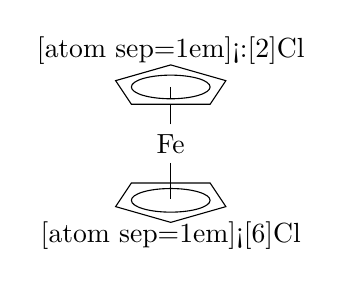
\begin{tikzpicture}
                \begin{scope}
                    \draw (0,0) -- (0.7,-0.2) -- (0.5,-0.5) -- (-0.5,-0.5) -- (-0.7,-0.2) -- cycle;
                    \draw (0,-0.28) ellipse (0.5cm and 0.15cm);
                \end{scope}
                \begin{scope}[yshift=-2cm,yscale=-1]
                    \draw (0,0) -- (0.7,-0.2) -- (0.5,-0.5) -- (-0.5,-0.5) -- (-0.7,-0.2) -- cycle;
                    \draw (0,-0.28) ellipse (0.5cm and 0.15cm);
                \end{scope}
                \node at (0,-1) {Fe}
                    edge (0,-1.7)
                    edge (0,-0.5)
                    (0,-0.28) edge (0,-0.43)
                ;
                \node [anchor=south] at (0,-0.12) {\chemfig[atom sep=1em]{<:[2]Cl}};
                \node [anchor=north] at (0,-1.87) {\chemfig[atom sep=1em]{<[6]Cl}};
            \end{tikzpicture}
            \vspace{1em}
        \end{center}
        \begin{proof}[Answer]
            Not low or high symmetry. Has a $C_2$ axis. No perpendicular $C_2$ axes. Has a $\sigma_h$\par
            Therefore, the above molecule is of the $C_{2h}$ point group.
        \end{proof}
        \item \ce{POCl3}
        \begin{proof}[Answer]
            Not low or high symmetry. Has a $C_3$ axis. No perpendicular $C_2$ axes. No $\sigma_h$. Has three $\sigma_v$ planes all offset by $\ang{60}$.\par
            Therefore, \ce{POCl3} is of the $C_{3v}$ point group.
        \end{proof}
        \item Tennis ball (including the seam)
        \begin{proof}[Answer]
            Not low or high symmetry. Has a $C_2$ axis. No perpendicular $C_2$ axes. No $\sigma_h$. Has two perpendicular $\sigma_v$ planes.\par
            Therefore, a tennis ball is of the $C_{2v}$ point group.
        \end{proof}
        \item \emph{trans}-\ce{[CrCl2(H2O)4]+}
        \begin{proof}[Answer]
            Not low or high symmetry. Has a $C_4$ axis. Has 4 perpendicular $C_2$ axes. Has $\sigma_h$.\par
            Therefore, \emph{trans}-\ce{[CrCl2(H2O)4]+} is of the $D_{4h}$ point group.
        \end{proof}
        \item 1,3,5-trichlorobenzene.
        \begin{proof}[Answer]
            Not low or high symmetry. Has a $C_3$ axis. Has 3 perpendicular $C_2$ axes. Has $\sigma_h$.\par
            Therefore, 1,3,5-trichlorobenzene is of the $D_{3h}$ point group.
        \end{proof}
        \item \emph{trans}-\ce{Pt(NH3)2Cl2}
        \begin{proof}[Answer]
            Not low or high symmetry. Has a $C_2$ axis. Has 2 perpendicular $C_2$ axes. Has $\sigma_h$.\par
            Therefore, \ce{TeF4^2-} is of the $D_{2h}$ point group.
        \end{proof}
        \item \ce{SF5Cl}
        \begin{proof}[Answer]
            Not low or high symmetry. Has a $C_4$ axis. No perpendicular $C_2$ axes. No $\sigma_h$. Has two perpendicular $\sigma_v$ planes and two perpendicular $\sigma_d$ planes.\par
            Therefore, \ce{SF5Cl} is of the $C_{4v}$ point group.
        \end{proof}
        \item \ce{BFClBr}
        \begin{proof}[Answer]
            \ce{BFClBr} is of the $C_s$ point group.
        \end{proof}
        \item \ce{PF2+}
        \begin{proof}[Answer]
            Not low or high symmetry. Has a $C_2$ axis. No perpendicular $C_2$ axes. No $\sigma_h$. Has two perpendicular $\sigma_v$ planes.\par
            Therefore, \ce{PF2+} is of the $C_{2v}$ point group.
        \end{proof}
    \end{enumerate}
    \newpage
    \item In the octahedral ion \ce{FeF6^3-}, what symmetry elements are destroyed if two \emph{trans} \ce{F} ions are moved away from the \ce{Fe^3+} center in an equidistant fashion?
    \begin{proof}[Answer]
        If the described change is made, the point group changes from $O_h$ to $D_{4h}$. In this change, every $C_3$ and $S_6$ axis, two of the three $C_4$ axes, and every $\sigma_d$ that does not contain the axis along which the \ce{F} ions are stretched are destroyed.
    \end{proof}
\end{enumerate}




\end{document}